\documentclass[runningheads,a4paper]{llncs}

\usepackage[latin1]{inputenc}
\usepackage{amssymb}
\usepackage{amsmath}
\setcounter{tocdepth}{3}
\usepackage{graphicx}
\usepackage{multirow}
\usepackage{rotating}
\usepackage{subfigure}
%\usepackage{subfig}
\usepackage{url}
\usepackage{caption}

\newcommand{\keywords}[1]{\par\addvspace\baselineskip
\noindent\keywordname\enspace\ignorespaces#1}

\providecommand{\tabularnewline}{\\}

\begin{document}

\mainmatter  % start of an individual contribution

% first the title is needed
\title{Addressing high dimensional multi-objective optimization problems by coevolutionary overlapped islands} %TITULO PROVISIONAL

% a short form should be given in case it is too long for the running head
\titlerunning{Addressing high dimensional multi-objective optimization problems}

% the name(s) of the author(s) follow(s) next
%
% NB: Chinese authors should write their first names(s) in front of
% their surnames. This ensures that the names appear correctly in
% the running heads and the author index.
%
%\author{P. Garc\'ia-S\'anchez \and J. Ortega \and
%  J. Gonz\'alez\inst{1} \and P. A. Castillo \and J.J. Merelo}
\author{A. U. Thor\inst{1}}
% �Se puede ayudar aqu�?
%
%\authorrunning{P. Garc\'ia-S\'anchez et al.}
\authorrunning{A. U. Thor}
% (feature abused for this document to repeat the title also on left hand pages)

% the affiliations are given next; don't give your e-mail address
% unless you accept that it will be published
%\institute{Dept. of Computer Architecture and Technology, University
%of Granada, Spain}
\institute{MIT, Midgardian Institute of Technology}

%
% NB: a more complex sample for affiliations and the mapping to the
% corresponding authors can be found in the file "llncs.dem"
% (search for the string "\mainmatter" where a contribution starts).
% "llncs.dem" accompanies the document class "llncs.cls".
%




\maketitle

%
%%%%%%%%%%%%%%%%%%%%%%%%%%%%%%%   ABSTRACT   %%%%%%%%%%%%%%%%%%%%%%%%%%%%%%%
%
\begin{abstract}
Large-scale multi-objective optimization problems with many decision variables have 
recently attracted attention as many data mining applications involving high 
dimensional patterns can take advantage of multi-objective approaches. Present 
parallel and distributed computer architectures can provide the required computing 
capabilities to cope with these problems once efficient procedures are available. In this 
paper we propose a cooperative coevolutionary island-model procedure based on the parallel 
execution of sub-populations, whose individuals explore different domains of the 
decision variables space. More specifically, the individuals belonging to the same 
sub-population (island) explore the same subset of decision variables. Two alternatives to 
distribute the decision variables among the different sub-populations have been 
considered and compared here. In the first approach, individuals in different 
sub-population explore disjoint subsets of decision variables (i.e. the chromosomes are 
divided into disjoints subsets). Otherwise, in the second alternative there are some 
overlapping among the variables explored by individuals in different sub-populations. 
The analysis of the obtained experimental results, by using different 
metrics, shows that coevolutionary approaches provide statistically significant 
improvements with respect to the base algorithm, being the relation of the number of 
islands (subpopulations) to the length of the chromosome (number of decision 
variables) a relevant factor to determine the more efficient alternative to distribute the 
decision variables.

\keywords{Multi-objective algorithms, NSGA-II, Island model, distributed evolutionary algorithms}
\end{abstract}

%
%%%%%%%%%%%%%%%%%%%%%%%%%%%%%%%   INTRODUCTION   %%%%%%%%%%%%%%%%%%%%%%%%%%%%%%%
%
\section{Introduction}

Evolutionary Algorithms (EAs) are inherently parallelizable, as each
individual can be considered as an independent unit
\cite{Alba13parallel}, and therefore, the
computational performance can be improved over their non-parallel
versions. This can also be applied to Multi-Objective Evolutionary 
Algorithms (MOEAs). Besides, as this kind of algorithms may be computationally
expensive, several parallelization methods have been proposed
\cite{Luna15Survey}. However, as MOEAs deal with whole solution sets
called Pareto Fronts (PFs), different distribution and sharing
mechanisms need to be addressed. Classic approaches, such as the
global parallel EAs (Master-Slave), or the spatially structured
algorithms (Island model or Cellular EAs) have been applied successfully in the past.   % this is a lot of boilerplate - JJ FERGU: Yes, I stil lhave to rewrite it

MOEAs have gained attention in the last years, mostly because their application in real-world problems \cite{Luna15Survey,Mukhopadhyay14Survey}. Usually these problems require a higher number of decision variables, and these larger individuals require a significant extra time for crossover, mutation and transmission. Therefore, dividing the decision space (that is, the chromosome) may improve high performance and solution quality. In this aspect, the co-evolution model is a dimension-distributed model where a
high-dimensional problem is divided into lower dimensional problems
\cite{Gong15models}, and evolved separately. Also, applying parallelism techniques in EAs not only implies a reduction in the execution time, 
but developing new and more efficient search models \cite{Luna15Survey}.  The idea of dividing the decision space has been
studied in \cite{Kimovski15Parallel}. In that work, different workers
evolve sub-populations created and recombined by a master process,
which performs different recombination alternatives from the parts returned by
worker processes. A high dimensional problem was used to compare these
alternatives. In \cite{Dorronsoro13superlinear}, a distributed coevolutionary island model was used.  In both previous works
significant speedups were attained, although only a low number of nodes were used (8). However, when increasing the number of islands, the division of each section of the chromosome becomes smaller, and the scalability may be affected by obtaining lower quality solutions in the same amount of time.
%In this paper, several of these ideas are taken into account to compare different approaches in
%chromosome division in distributed island MOEAs. 

The hypothesis of this paper is that using overlapped sections of the chromosome in a coevolutionary multi-objective island-based algorithm can improve the quality of the
solutions in the same computing time when the number of islands increases. To demonstrate this, a new overlapping islands scheme will be compared with a baseline version of a distributed NSGA-II \cite{Deb00NSGAII} and with a coevolutionary disjoint section approach, in different benchmarks problems and with different large number of islands. Results show that this new technique can improve different quality indicators in
the same amount of time. 

The rest of the paper is structured as follows: after a background in parallelization in MOEAs, 
 the compared algorithms and the used methodology (Section \ref{sec:met}) are presented. 
Then, the results of the experiments are shown (Section \ref{sec:res}), followed by conclusions and suggestions for future work lines.


%%%%%%%%%%%%%%%%%%%%%%%%%%%%%%  STATE OF THE ART  %%%%%%%%%%%%%%%%%%%%%%%%%%%%%
%
\section{State of the Art}
\label{sec:soa}

%make it a narrative. - JJ FERGU: I know, I know, it was still pending :) TODO
Distributed and parallel Evolutionary Algorithms have been used since
the early 2000s \cite{Talbi08Parallel} to leverage the capabilities of new common parallel computer architectures, such as
clusters or grids. However, distributing MOEAs is not as easy as it is
in single-objective EAs, as they have to deal with a whole set of dependent solutions, the Pareto Front, that should be managed in several steps of the algorithm. %unfinished Pablo: Done
Some authors have focused on Master-Slave approaches to parallelize this kind of EAs. For example, Durillo et
al. \cite{Durillo08masterslave} compared different master-slave
approaches to save time when running the EA. The method proposed by
Hiroyasu \cite{Hiroyasu07discussion} generates offspring depending on
the computation power.  

%Dividing the decision or search space of EAs in different islands is
%not a novel idea \cite{ALGUNOANTIGUO}. However, when using
%multi-objective EAs ... 

First approaches for distributed MOEAs (dMOEAs) were studied in
\cite{Deb03distributed}. In that work, the dominance of solutions is
divided in the islands using a transformation of coordinates. Authors
concluded that dividing the search space is a good idea, but achieve
this is not trivial. Other ideas for dividing the search space include
objective separation in different processors \cite{Xiao03specialized},
or divide in two populations: one for elite and other search
\cite{Wang09parallel}. Martens, in \cite{Martens13asynchronous} used a
Barabasi-Albert island topology and selection based on migrating
individuals from a not-crowded area and acceptance based on
diversity. 

More similar approaches to the one presented here were studied in the
 next two works, also using cooperative coevolution for high-dimensional problems. Dorronsoro et al. in
\cite{Dorronsoro13superlinear} obtained super-linear performance
in several instances using cooperative coevolution, focusing each island on a portion of the chromosome. However, in some instances the parallel version not always 
improved the sequential version.  Kimovski et al. \cite{Kimovski15Parallel} proposed a
master-slave method that splits the population into several processors,
each one running in parallel a MOEA that only affects some portion of
the individuals. After a certain number of generations, the master
process receives all the sub-populations to be combined. Different
combination alternatives in this step are compared. Up to 8 processors
were used in the experimental setup. Our approach in this paper does not
broadcast all solutions to all islands for recombination, as previous
works, but only one solution to a random island, needing less
communication time. Besides, the maximum number of islands of
Dorronsoro or Kimovsky approaches was 8, while in this paper we have
used up to 128 islands. 




%
%%%%%%%%%%%%%%%%%%%%%%%%%%%%%%  METHODOLOGY  %%%%%%%%%%%%%%%%%%%%%%%%%%%%%
%
\section{Methodology and experimental setup}
\label{sec:met}
This section describes the quality indicators used and the methods compared. The chosen quality indicators are:

\begin{itemize}
\item Hypervolume (HV): measures the area formed by all non-dominated solutions found with, respect to a reference point. 
\item Inverted Generational distance (IGD): calculates the distance of the obtained set of solutions to the optimal PF. Therefore, this metric requires the optimal PF found in the literature, or the theoretical one. %Pablo: theoretical?
\item Spread (S): Measures the spread between solutions, taking into account the euclidean distance between consecutive solutions.
\end{itemize}

With exception of the HV, the lower, the better. All these metrics have been used and described in previously presented works \cite{Deb03distributed,Durillo08masterslave,Hiroyasu07discussion,Dorronsoro13superlinear} in Section \ref{sec:soa}.


% --------------------------------------------------------------

\subsection{Baseline algorithm}
This algorithm is a regular NSGA-II algorithm distributed along a number $P$ of islands. Every certain number of generations, one individual is migrated to another random island. At the end of the run, all PFs of all islands are aggregated in a new one and the metrics are calculated.


\subsection{Disjoint Algorithm}

In this approach, each individual of size $L$ is split into $P$ chunks of size $L/P$. Every island $p$ only performs crossover and mutation on the $p_{th}$ part of the individuals.  As in the baseline, every certain number of generations, an individual is migrated to another random island.  In the new island, this individual will be crossed and mutated as the other individuals on the island. Note that, on the contrary of other works such as the ones described \cite{Talbi08Parallel} all the islands deal with complete chromosomes for fitness calculation, so our approach can deal with no decomposable problems. Figure \ref{fig:disjoint} describes this approach, with $P=5$ islands.

\begin{figure}
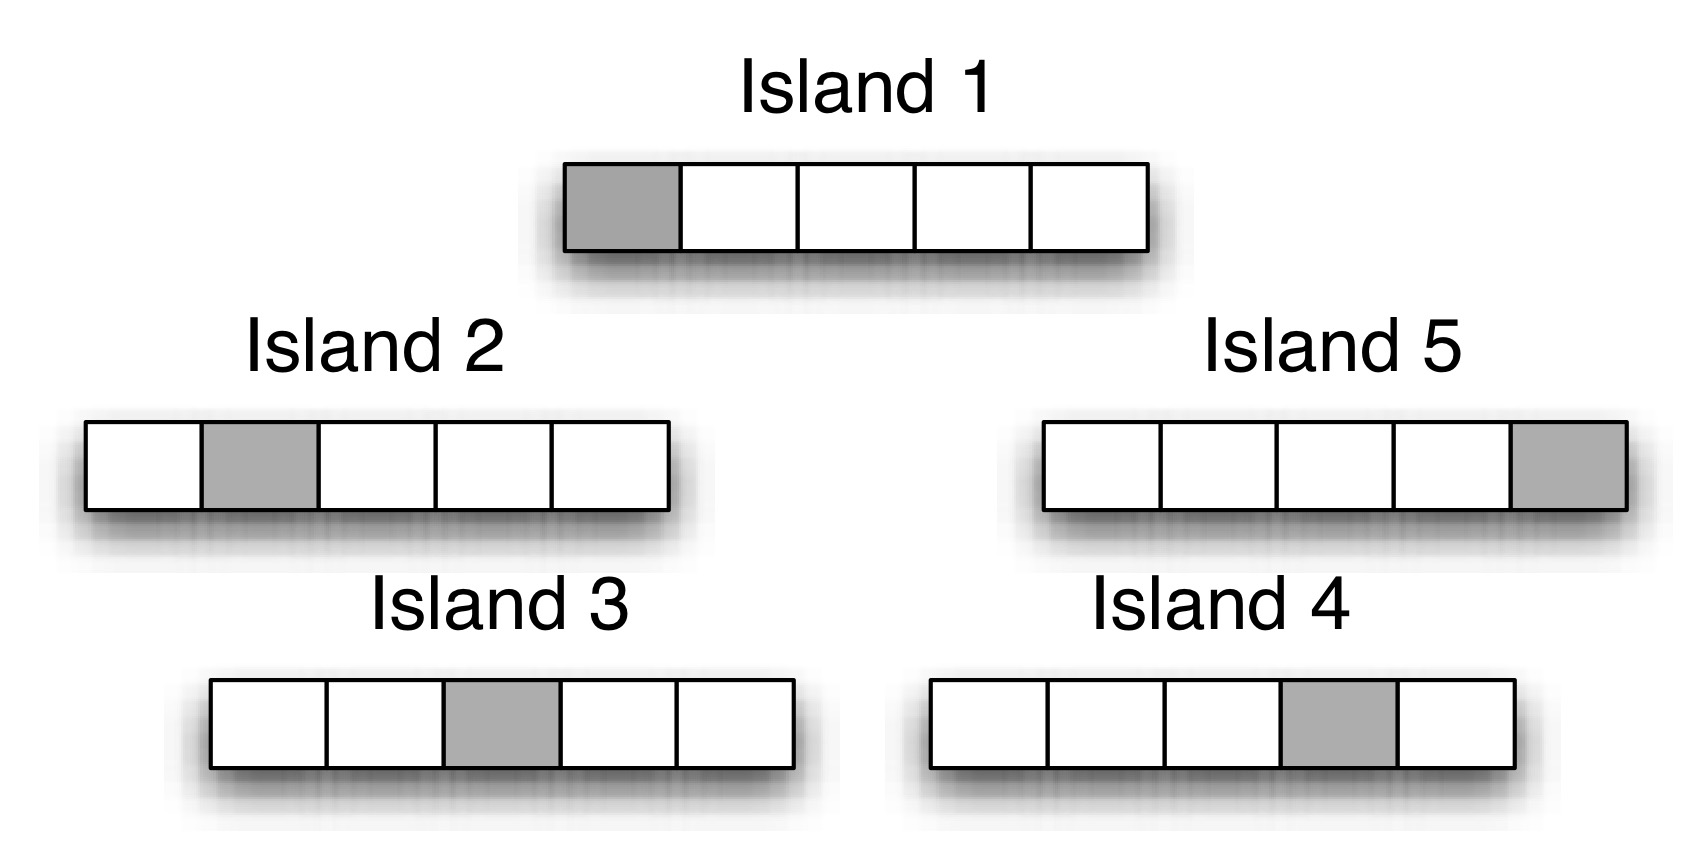
\includegraphics[width=10cm]{islandDisjoint.jpg}
\caption{Disjoint algorithm: every island $p$ only modifies the $p_{th}$ part (in grey) of the individuals.}
\label{fig:disjoint}
\end{figure}

\subsection{Overlapped Algorithm}
This approach is similar to the previous one, but every island also uses the $p+1$ and $p-1$ (module size) chunks of the individual for crossover and migration. Therefore, some kind of overlapping of the crossed and mutated parts exists between islands. Figure \ref{fig:overlapped} shows the affected parts of the individuals in each island.

 
\begin{figure}
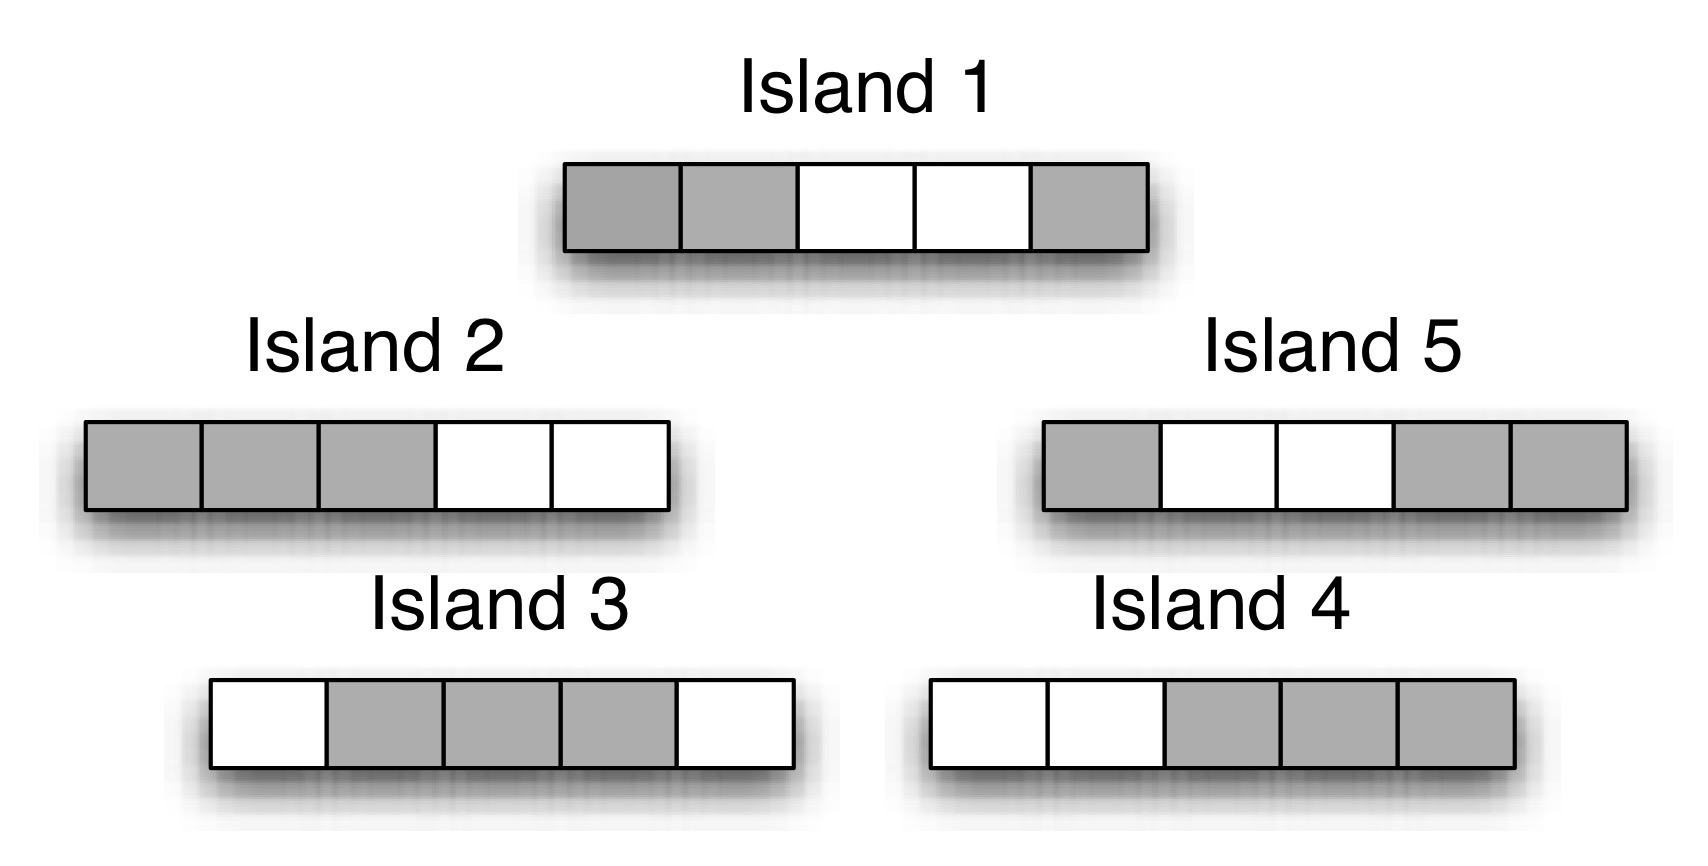
\includegraphics[width=10cm]{islandNoDisjoint.jpg}
\caption{Disjoint algorithm: every island $p$ modifies the  $p+1$, $p_{th}$ and $p-1$  parts (in grey) of the individuals.}
\label{fig:overlapped}
\end{figure}

% --------------------------------------------------------------


%%%%%%%%%%%%%%%%%%%%%%%%%%  EXPERIMENTS AND RESULTS  %%%%%%%%%%%%%%%%%%%%%%%%%%
%
\section{Experiments and Results}
\label{sec:res}

The three approaches have been launched with a different combination of chromosome lengths ($L$): 512 and 2048. Also, different number of islands ($P$) have been compared: 8, 32 and 128. This maximum number of islands have been also used in previous work in the literature \cite{Martens13asynchronous}. The crossover and mutation chosen, SBX and polynomial, have been used previously by other authors in \cite{Durillo08masterslave}.

The chosen problems to evaluate are the ZDT. This benchmark has been chosen because it has been previously used in different works of the literature \cite{Deb03distributed,Martens13asynchronous,Wang09parallel,Durillo08masterslave}. The optimal PF distribution used for comparison has 1000 solutions \footnote{Optimal PFs can be obtained here: \url{http://www.tik.ee.ethz.ch/sop/download/supplementary/testproblems/}.}.





The termination criterion used is the execution time: 25 seconds for dimension 512 and 100 (four times more) for 2048. We have used the time instead the number of evaluations firstly because our hypothesis argue that the time saved in crossover in mutation can be spent on improving the sub-populations and more operations and migrations can be achieved. Also, we are using different number of islands (with different sub-population sizes) that could lead to different execution times, so it would be difficult to compare different times and quality solutions at the same time.

\begin{table}
\begin{center}
\begin{tabular}{|c|c|}
\hline
{\em Parameter Name} & {\em Value} \\ \hline
Number of islands ($P$) & 8, 32 and 128 \\ \hline
Chromosome size ($L$) & 512 and 2048 \\ \hline
Execution time (s) & 25 (for 512) and 100 (for 2048) \\ \hline \hline
Global population size ($N$) & 1024 \\ \hline
Selection type & Binary Tournament Selection \\ \hline
Replacement type & Generational \\ \hline %FERGU: tiene sentido cuando hablamos de NSGA2?
Crossover type & SBX \\ \hline
Mutation  type & Polynomial\\ \hline
Mutation probability & 1/$L$ \\ \hline
Generations between migration & 5 \\ \hline
Individuals per migration & 1 \\ \hline
Selection for migration & Binary Tournament\\ \hline
Runs per configuration & 30 \\ \hline
\end{tabular}
\caption{Parameters and operators used in the experiments.}
\label{tab:parameters}
\end{center}
\end{table}

%%%FERGU: NO OLVIDAR PONER EL REPOSITORIO!!!!!!!!!!!!!!!!!!!!!!

The ECJ framework \cite{ECJ} has been used to run the experiments. Specific operators have been developed as new modules for ECJ, and they can be downloaded from our GitHub repository under a LGPL V3 License \footnote{\url{https://ANONYMOUS-REPOSITORY}}. The island model has been executed synchronously, using the ECJ Internal Island Model, in a CentOS 5.4 machine with Intel(R) Xeon(R) CPU E5520 @2.27GHz, 16 GB RAM, with Java Version 1.6.0\_16. As in this paper we only focus on the behaviour of our model in a non-real scenario (the islands share the same memory and processor), the migration time will not be as an important factor as in a real distributed system. This task will be addressed in future works. %Pablo: no s� si decir esto aqu�



Different metrics, explained in the previous section, have been used to calculate the quality of the obtained PFs in each configuration. As some of the metrics require a reference point to be calculated (such as HV), the point (1,9) has been chosen as reference, as none of the generated PFs in all runs are dominated by it. Metrics are then normalized with respect to that point. A Kruskall-Wallis significance test has been performed to the metrics of all runs of the configurations, as the Kolmogorov-Smirnov test detected non-normal distributions. The average results for each configuration are shown in Table \ref{tab:results}.

\begin{table}
\centering
\resizebox{12cm}{!}{
\begin{tabular}{|c||c|c|c||c|c|c||c|c|c||}
\hline %PON EL 0.000 a 0.0004
 
	&	\multicolumn{3}{|c|}{HV}								&	\multicolumn{3}{|c|}{Spread}								&	\multicolumn{3}{|c|}{IGD}								\\ \hline
\multicolumn{10}{|c|}{512 dimensions}																												\\ \hline
\#Islands	&	Baseline	&	Disjoint	&		Overlapped			&	Baseline	&	Disjoint		&	Overlapped			&	Baseline	&	Disjoint		&	Overlapped			\\ \hline
\multicolumn{10}{|c|}{ZDT1}																												\\ \hline
8	&	0.870	&	0.961	&		0.943			&	0.775	&	0.546		&	0.720	*		&	0.019	&	0.000		&	0.004			\\
32	&	0.803	&	0.887	&		0.957			&	0.815	&	0.837	*	&	0.621			&	0.033	&	0.014		&	0.001			\\
128	&	0.744	&	0.687	&		0.827			&	0.850	&	0.874	*	&	0.839	*		&	0.045	&	0.054		&	0.024			\\ \hline
\multicolumn{10}{|c|}{ZDT2}																												\\ \hline
8	&	0.787	&	0.919	&		0.878			&	0.913	&	0.646		&	0.907	*		&	0.035	&	0.001		&	0.011			\\
32	&	0.744	&	0.890	&		0.917			&	0.950	&	0.754		&	0.627			&	0.048	&	0.007		&	0.002			\\
128	&	0.693	&	0.592	&		0.765			&	0.971	&	0.944		&	0.917		$\bullet$	&	0.062	&	0.089		&	0.039			\\ \hline
\multicolumn{10}{|c|}{ZDT3}																												\\ \hline
8	&	0.894	&	0.976	&		0.965			&	0.895	&	0.832		&	0.922	*		&	0.012	&	0.001		&	0.003			\\
32	&	0.829	&	0.902	&		0.972			&	0.877	&	0.851		&	0.835			&	0.019	&	0.011		&	0.001			\\
128	&	0.770	&	0.726	&		0.865			&	0.891	&	0.845		&	0.845		$\bullet$	&	0.026	&	0.029		&	0.015			\\ \hline
\multicolumn{10}{|c|}{ZDT6}																												\\ \hline
8	&	0.224	&	0.503	&		0.331			&	0.992	&	1.008	*	&	0.993	*	$\bullet$	&	0.192	&	0.070		&	0.145			\\
32	&	0.192	&	0.396	&		0.454			&	0.998	&	0.998	*	&	0.980	*	$\bullet$	&	0.206	&	0.118		&	0.091			\\
128	&	0.157	&	0.114	&		0.214			&	1.004	&	0.985		&	0.979		$\bullet$	&	0.221	&	0.238		&	0.195			\\ \hline
																												
																												
																												
																												
																												
	&	\multicolumn{3}{|c|}{HV}								&	\multicolumn{3}{|c|}{Spread}								&	\multicolumn{3}{|c|}{IGD}								\\ \hline
\multicolumn{10}{|c|}{2048 dimensions}																												\\ \hline
\#Islands	&	Baseline	&	Disjoint	&		Overlapped			&	Baseline	&	Disjoint		&	Overlapped			&	Baseline	&	Disjoint		&	Overlapped			\\ \hline
\multicolumn{10}{|c|}{ZDT1}																												\\ \hline
8	&	0.754	&	0.948	&		0.889			&	0.844	&	0.587		&	0.807	*		&	0.044	&	0.003		&	0.015			\\
32	&	0.679	&	0.928	&		0.942			&	0.854	&	0.714		&	0.646			&	0.061	&	0.006		&	0.004			\\
128	&	0.660	&	0.765	&		0.907			&	0.865	&	0.860	*	&	0.802			&	0.065	&	0.036		&	0.010			\\ \hline
\multicolumn{10}{|c|}{ZDT2}																												\\ \hline
8	&	0.641	&	0.877	&		0.794			&	0.965	&	0.942		&	0.969	*	$\bullet$	&	0.078	&	0.011		&	0.033			\\
32	&	0.605	&	0.898	&		0.885		$\bullet$	&	0.980	&	0.704		&	0.755		$\bullet$	&	0.088	&	0.006		&	0.009		$\bullet$	\\
128	&	0.560	&	0.689	&		0.830			&	0.984	&	0.929		&	0.870			&	0.101	&	0.060		&	0.021			\\ \hline
\multicolumn{10}{|c|}{ZDT3}																												\\ \hline
8	&	0.773	&	0.969	&		0.922			&	0.910	&	0.865		&	0.919		$\bullet$	&	0.026	&	0.002		&	0.009			\\
32	&	0.713	&	0.937	&		0.966			&	0.903	&	0.796		&	0.839			&	0.032	&	0.007		&	0.002			\\
128	&	0.691	&	0.817	&		0.935			&	0.902	&	0.839		&	0.812		$\bullet$	&	0.035	&	0.020		&	0.007			\\ \hline
\multicolumn{10}{|c|}{ZDT6}																												\\ \hline
8	&	0.136	&	0.334	&		0.231			&	0.995	&	1.002		&	0.996	*	$\bullet$	&	0.230	&	0.144		&	0.189			\\
32	&	0.113	&	0.394	&		0.327			&	0.996	&	0.975		&	0.990	*	$\bullet$	&	0.240	&	0.118		&	0.147			\\
128	&	0.101	&	0.165	&		0.267			&	0.997	&	0.985		&	0.979		$\bullet$	&	0.245	&	0.216		&	0.172			\\ \hline


\end{tabular}
}
\caption{Quality metrics obtained after 30 runs per configuration, for the three methods compared: Baseline, Disjoint  and Overlapped. An asterisk (*) means that there is not significant difference with respect to Baseline, and a bullet ($\bullet$) indicates there is not difference between Disjoint and Overlapped.}
\label{tab:results}
\end{table}

At a first glance results show that dividing the chromosome produces an improvement in all the quality indicators in all the configurations, with respect to the baseline. Also, results also show that all the quality indicators lowers when the number of islands is increased, as the subpopulations are smaller. This is consistent with the claim by Durillo in \cite{Dorronsoro13superlinear}, where cooperative coevolutionary MOEAs work better on bigger populations (more than 100 individuals). With respect to the disjoint and overlapped methods, when using 8 islands the disjoint method always attain better metrics, and more times with the 2048 chromosome length. This can be explained because only 1/8 of the individual is changed in each island, while in the overlapped, 3/8 of the island may be more similar to the baseline. Therefore, there exist some kind of limit point where one method will be preferable to another, depending the number of islands, population size and length.

This can be explained also comparing the number of generations and average solutions per island. Table \ref{tab:gens} shows these values obtained in each method. It is clear that in the same amount of time, the disjoint and overlapped method attains more generations than the baseline. This is even clearer with $L=$2048, where almost 10 times the number of generations is attained, and therefore, more migrations and crossovers/mutations can be achieved. Surprisingly, the average number of solutions of PFs per island in the baseline is significantly higher in some configurations (mostly with 128 islands), but their combination in the final PF never attains higher values than Disjoint and Overlapped methods.

\begin{table}
\centering
\begin{tabular}{|c||c|c|c||c|c|c||}
\hline
	&	\multicolumn{3}{|c|}{Generations}								&	\multicolumn{3}{|c|}{Avg. solutions per island}								\\ \hline
\multicolumn{7}{|c|}{512 dimensions}																			\\ \hline
\#Islands	&	Baseline	&	Disjoint	&		Overlapped			&	Baseline	&	Disjoint		&	Overlapped			\\ \hline
\multicolumn{7}{|c|}{ZDT1}																			\\ \hline
8	&	112.933	&	453.333		&	225.233			&	118.733	&	137.000		&	141.467		$\bullet$	\\
32	&	111.333	&	851.933		&	561.667			&	69.433	&	33.067		&	73.833	*		\\
128	&	126.433	&	607.200		&	606.533			&	62.367	&	18.200		&	25.567			\\ \hline
\multicolumn{7}{|c|}{ZDT2}																			\\ \hline
8	&	110.333	&	426.033		&	222.667			&	42.233	&	122.500		&	101.367			\\
32	&	113.300	&	801.800		&	595.267			&	28.800	&	26.600	*	&	62.367			\\
128	&	134.300	&	615.467		&	595.733		$\bullet$	&	20.300	&	11.433		&	13.200		$\bullet$	\\ \hline
\multicolumn{7}{|c|}{ZDT3}																			\\ \hline
8	&	106.967	&	449.533		&	227.467			&	143.933	&	138.167	*	&	160.967	*		\\
32	&	113.500	&	819.533		&	554.767			&	90.033	&	38.200		&	69.767			\\
128	&	122.633	&	630.533		&	596.300			&	70.167	&	17.933		&	25.133			\\ \hline
\multicolumn{7}{|c|}{ZDT6}																			\\ \hline
8	&	109.767	&	435.800		&	215.833			&	16.933	&	35.533		&	17.367	*		\\
32	&	113.267	&	720.233		&	518.733			&	15.800	&	11.233		&	15.100	*	$\bullet$	\\
128	&	131.333	&	597.200		&	569.500			&	15.367	&	8.467		&	8.533	 	$\bullet$	\\ \hline
																			
																			
																			
																			
																			
	&	\multicolumn{3}{|c|}{Generations}								&	\multicolumn{3}{|c|}{Avg. solutions per island}								\\ \hline
\multicolumn{7}{|c|}{2048 dimensions}																			\\ \hline
\#Islands	&	Baseline	&	Disjoint	&		Overlapped			&	Baseline	&	Disjoint		&	Overlapped			\\ \hline
\multicolumn{7}{|c|}{ZDT1}																			\\ \hline
8	&	118.333	&	574.100		&	262.700			&	136.167	&	126.267		&	136.267	*	$\bullet$	\\
32	&	115.567	&	1195.800		&	721.733			&	103.867	&	35.000		&	60.267			\\
128	&	141.067	&	1266.700		&	1170.767			&	98.000	&	20.167		&	30.467			\\ \hline
\multicolumn{7}{|c|}{ZDT2}																			\\ \hline
8	&	111.833	&	584.233		&	265.933			&	32.100	&	86.600		&	78.067		$\bullet$	\\
32	&	121.367	&	1278.700		&	757.667			&	25.600	&	41.833		&	45.133		$\bullet$	\\
128	&	143.567	&	1306.700		&	1133.367			&	22.967	&	12.767		&	20.800	*		\\ \hline
\multicolumn{7}{|c|}{ZDT3}																			\\ \hline
8	&	111.700	&	589.800		&	265.567			&	167.633	&	129.333		&	144.000			\\
32	&	117.633	&	1154.133		&	772.633			&	129.167	&	36.667		&	72.767			\\
128	&	136.267	&	1379.067		&	1128.467			&	105.767	&	19.367		&	29.400			\\ \hline
\multicolumn{7}{|c|}{ZDT6}																			\\ \hline
8	&	116.867	&	585.333		&	267.133			&	22.867	&	27.267	*	&	32.600			\\
32	&	118.533	&	1082.633		&	684.500			&	22.133	&	12.067		&	16.633		$\bullet$	\\
128	&	162.267	&	1296.733		&	1102.867			&	20.167	&	7.400		&	9.267		$\bullet$	\\ \hline



\end{tabular}
\caption{Number of generations and average number of solutions per island obtained after 30 runs per configuration, for the three methods compared: Baseline, Disjoint and Overlapped. An asterisk (*) means that there is not significant difference with respect to Baseline, and a bullet ($\bullet$) indicates there is not difference between Disjoint and Overlapped.}
\label{tab:gens}
\end{table}

\section{Conclusions}

High-performance problems that require a large number of decision variables can leverage from dividing the decision space in parallel and distributed algorithms. This can be applied in dMOEAs dividing the chromosome in different parts, each one modified in a different island. This paper compares a baseline distributed NSGA-II with two different methods to separate the chromosome (disjoint or overlapped parts). Results show that these methods can achieve better results than the baseline, being the relation of the number of islands used and the length of the chromosome a key factor to decide to take advantage of these methods. This can be explained because the time reduction in crossover and mutation in the chromosomes.

In future work, other MOEAs, such as SPEA will be compared, with more configurations of population size and chromosome lengths. Also, a real distributed system (such as a GRID or cluster) with more different numbers of islands/processors, will be used to compare the different methods, and a scalability study will be performed, therefore the transmission time between islands will also be a relevant issue to study. New benchmarks and real problems will be also used to validate our approach.


\section*{Acknowledgments} %PONER EL DEL NUEVOOOOOO Y EL DE MARIBEL EN INGLES!!!!
Hidden for double blind review 
%\scriptsize{This work has been supported in part by SIPESCA (Programa Operativo FEDER de Andaluc\'ia 2007-2013), TIN2011-28627-C04-02 (Spanish Ministry of Economy and Competitivity), SPIP2014-01437 (Direcci\'on General de Tr\'afico), PRY142/14 (Fundaci\'on P\'ublica Andaluza Centro de Estudios Andaluces en la IX Convocatoria de Proyectos de Investigaci\'on) and PYR-2014-17 GENIL project (CEI-BIOTIC Granada).}


%
%Hidden for double-blind review


\bibliographystyle{splncs}
\bibliography{hpmoon-evostar}


\end{document}
